% LaTeX template for a short report (written for MSES scenario modelling)
% uses LaTeX documentclass "article" for use of sections (not chapter) and References (not Bibliography)
% for Chapters and Bibliography use "documentclass "report
\documentclass[10pt]{article}   % Use article class with 10pt letter
%\documentclass[10pt]{report}
\usepackage[utf8]{inputenc}

%\usepackage[T1]{fontenc}  % 8-bit encoding, helps hyphenation of accented characters -
% https://tex.stackexchange.com/a/677/42066

% Use A4 paper and set margins:
%\usepackage[a4paper, twoside, top=2.0cm, left=3.0cm, bottom=2.0cm, right=2.0cm]{geometry}
\usepackage[a4paper, twoside, top=2.0cm, left=2.0cm, bottom=2.0cm, right=2.0cm]{geometry}
%\usepackage[a4paper, top=2.5cm, left=2.5cm, bottom=2.5cm, right=2.5cm]{geometry}

\usepackage[english]{babel}  % Hyphenation and more for English

\usepackage{pgf}      % Include graphics inside figures using \pgfimage
\usepackage[font=small, labelfont=bf]{caption}  % Stylize figure, table, etc. captions

\usepackage{parskip}         % Replace paragraph indentations with white lines
\usepackage[hyphens]{url}    % Take care of urls, e.g. wrapping in the Bibliography (hyphens: also break at -)

\usepackage{xspace}   % \xspace saves the user from having to type \  or {} after a macro name in text.

% Use the appendix package for nicer appendices:
%\usepackage[toc,page]{appendix}  % MvdS
\usepackage[titletoc]{appendix}
%\usepackage[toc,page,title]{appendix}  % Use \begin{appendices} ... \end{} iso \appendix

% \usepackage[numbib,numindex]{tocbibind}  % Add ToC, List of Figures/Tables/Code listings, Bibliography and Index to ToC
% \usepackage[]{tocbibind}       % Add ToC, List of Figures/Tables/Code listings, Bibliography and Index to ToC
\usepackage[nottoc]{tocbibind}   % ToC without extra "Contents" entry...

\usepackage{amsmath,amssymb,bbm}
\usepackage{enumerate}         % Choose alternative numberings, e.g. \begin{enumerate}[a.]

\usepackage{listings}          % Code listings
\usepackage[section, above, below]{placeins}  % \FloatBarrier - flush floats before \section by default
% \usepackage{pgf}               % Figures

\usepackage{color}
\definecolor{lightgrey}{rgb}{0.9,0.9,0.9}
\definecolor{darkgreen}{rgb}{0.0,0.6,0.0}

% Citations:

% option1: use natbib/bibtex with MvdS_number_url.bst
%\usepackage[numbers, square]{natbib}  % Use numbered citations with square brackets
%\bibliographystyle{MvdS_number_url}  % Use [1], print url = field  (plain doesn't print urls)

%option2: use biblatex/biber without *.bst file
\usepackage[backend=biber, style=numeric, citestyle=numeric-comp, sorting=none]{biblatex} 
\setlength\bibitemsep{0.5\baselineskip}
\usepackage{csquotes}

% \bibliography{mybibliography} % old-style for backward comp. in preamble for biblatex/bibtex
\addbibresource{mybibliography.bib}  % new syntax for BibLaTeX


\usepackage{fancybox}  % Use \ovalbox for key strokes

\newcommand{\ldf}{\usefont{OT1}{cmr}{m}{n}}     % Select default LaTeX font - Computer Modern Roman
%\newcommand{\ldf}{\usefont{OT1}{cmss}{m}{n}}     % Select default LaTeX font - Computer Modern Sans
%\newcommand{\ldf}{\usefont{OT1}{phv}{m}{n}}     % Select default LaTeX font - Helvetica
\newcommand{\ttbf}{\usefont{OT1}{lmtt}{bx}{n}}  % Select bold typewriter font

%\usepackage[font=sf]{caption}  % Use sans-serif font for float captions - not exactly Helvetica



\newcommand{\note}[1]{\color{red}\textbf{#1}\color{black}\xspace}
\newcommand{\marc}[1]{\color{red}\textbf{Marc: #1}\color{black}\xspace}

\newcommand{\myChapter}[1]{
  \chapter{#1}
  \minitoc  % Create a ToC of this chapter
}


% General expressions:
\newcommand{\eg}{\emph{e.g.}\xspace}
\newcommand{\ie}{\emph{i.e.}\xspace}
\newcommand{\etc}{\emph{et cetera}\xspace}
\newcommand{\ff}{\emph{ff}\xspace}

% CLI symbols:
\newcommand{\pipe}{$|$}      % Needed to avoid | in \index{}
\newcommand{\logor}{$|\,|$}  % Needed to avoid | in \index{}
\newcommand{\home}{\url{~}}  % Home directory


% Often used code names:
\newcommand{\NULL}{\code{NULL}}
\newcommand{\void}{\code{void}}
\newcommand{\stdout}{\code{stdout}}
\newcommand{\stderr}{\code{stderr}}

% Man pages:
\newcommand{\man}[2]{\texttt{man #1 #2}\xspace}
\newcommand{\mancmd}[1]{\texttt{man #1}\xspace}

% Code:
\newcommand{\prototype}[3]{\hspace*{2em}\texttt{#1} {\ttbf #2\ldf}(\texttt{#3});\xspace}  % function prototype
\newcommand{\var}[2]{\hspace*{2em}\texttt{#1} {\ttbf #2\ldf};\xspace}  % variable declaration
\newcommand{\code}[1]{\texttt{#1}\xspace}  % inline code
\newcommand{\codeb}[1]{\ttbf #1\ldf\xspace}  % inline bold code
\newcommand{\codeline}[1]{\hspace*{2em}\texttt{#1}}  % separate code line

\newcommand{\cli}[1]{\noindent\hspace*{2em}\code{\$ #1}}  % command line input
\newcommand{\clir}[1]{\noindent\hspace*{2em}\code{\# #1}}  % command line input root
\newcommand{\clo}[1]{\noindent\hspace*{2em}\code{#1}}  % command line output
\newcommand{\clitem}[1]{\item[\code{\$}] \code{#1}}  % cli in itemized list, with $ as bullet
\newcommand{\clitemb}[1]{\item[\codeb{\$}] \codeb{#1}}  % cli in itemized list, with $ as bullet - bold

\newcommand{\key}[1]{\Ovalbox{\texttt{#1}}\xspace}  % key press/combination
\newcommand{\keyb}[1]{\Ovalbox{\ttbf #1\ldf}\xspace}  % key press/combination bold


% Heat pumps
\newcommand{\COP}{\mathrm{COP}}  % COP in "math mode"
\newcommand{\COPh}{\COP_{\mathrm{heating}}}  % COP_heating in "math mode"

\newcommand{\Qh}{Q_{\mathrm{H}}}
\newcommand{\Qc}{Q_{\mathrm{C}}}
\newcommand{\Th}{T_{\mathrm{H}}}
\newcommand{\Tc}{T_{\mathrm{C}}}

\newcommand{\Tin}{T_{\mathrm{in}}}
\newcommand{\Tout}{T_{\mathrm{out}}}

\newcommand{\Ph}{P_{\mathrm{heat}}}
\newcommand{\Pheat}{P_{\mathrm{heat}}}
\newcommand{\Pc}{P_{\mathrm{cool}}}
\newcommand{\Pcool}{P_{\mathrm{cool}}}
\newcommand{\Pel}{P_{\mathrm{el}}}

\newcommand{\degr}{^\circ}
\newcommand{\tdeg}{$\degr$\xspace}
\newcommand{\degC}{\degr\mathrm{C}}
\newcommand{\tdegC}{$\degC$\xspace}

  % Custom commands

\usepackage[pdftex]{hyperref}
\hypersetup{
  colorlinks = true,  % They get a red box around them if false, better set colour to black?
  linkcolor = blue,
  filecolor = magenta,
  citecolor = blue,
  urlcolor = blue,
  % linkcolor = black,
  % citecolor = black,
  % urlcolor = black,
  pdftitle = House Model References,
  pdfauthor = Trung Nguyen,
  pdfsubject = House Models,
  pdfkeywords = house - models - Python,
  pdfcreator = TeXStudio pdfLaTeX2 on Windows,
  pdfproducer = TeXStudio pdfLaTeX2 on Windows,
  bookmarksnumbered = true,  % Number sections in PDF toc
}

\usepackage[onehalfspacing]{setspace}
\usepackage{float}

\usepackage{graphicx}
\usepackage{multirow}

%\renewcommand{\thesection}{\arabic{section}}  % needed for documentclass "report" with sections






% Title page:
\title{House model}
\author{Trung Nguyen\\
HAN University of Applied Sciences\\
Arnhem, The Netherlands} %\\


\begin{document}
	
\ldf  % Set LaTeX default font

% Set up code listing style:
\lstset{
	language=Python,
	% Fonts:
	basicstyle=\ttfamily\footnotesize,
	%keywordstyle=\ttfamily,
	%identifierstyle=,
	%commentstyle=\ttfamily\scriptsize,
	% B/W code:
	% commentstyle=\ttfamily\itshape,  % Italic
	% stringstyle=\ttfamily,
	% identifierstyle=\ttbf,           % Bold typewriter type
	% keywordstyle=\ttbf,              % Bold tt
	% Colour:
	commentstyle=\scriptsize\ttfamily\color{brown},
	stringstyle=\ttfamily\color{darkgreen},
	identifierstyle=\color{blue},
	keywordstyle=\ttfamily\color{red},
	% Spaces:
	showstringspaces=false,
	breaklines=true,
	breakatwhitespace=true,
	% Line numbering:
	numbers=left,
	numberstyle=\tiny,
	stepnumber=2, 
	numbersep=5pt,
	% Frames:
	frame=single,
	frameround=tttt,
	backgroundcolor=\color{lightgrey},
	morekeywords={pthread_create},
}
%\renewcommand{\thelstlisting}{\thechapter.\arabic{lstlisting}}  % This is the default?
%\numberwithin{lstlisting}{section}  % AMSmath: number code listings per section
%\numberwithin{lstlisting}{chapter}  % AMSmath: number code listings per chapter


\maketitle

%\begin{center}
%	\today
%\end{center}

\tableofcontents

\newpage

% \chapter{Introduction}

\section{Introduction}

The report give an overview and compare between the available  PID and advance python control packages. The different PID forms will be discussed in section 2. In section 3 and 4 are the most used PID python packages in practice with their advantages and disadvantages. Finally section 5 give an overview on some advance control and optimization python library.


\newpage


\section{White box lumped model: RC network}
\subsection{White box lumped model}

The objective of the house model for this project is to serve as test environment for a heat pump model, which means that the house model is intended as a tool to help taking building systems design decisions. The house heating demand calculation model implemented for this project is a white box \emph{lumped} model. Specifically, it is a RC network model consisting of resistances (R) and capacities (C). The RC network model is based on the analogy with electrical circuits. The simulation of thermodynamic systems characterizing building elements as resistances or capacities allows to simplify the model while maintaining a high simulation results accuracy \textbf{(Bagheri et al.\cite{en11040890}, Bacher et al\cite{Bacher}.)}.  

There are several types of RC models, the most common being 3R4C models and 3R2C models which are applied on the outer and internal wall. For the simulation of simple house buildings 3R2C models perform as accurate as more complex 3R4C models \textbf{(Fraisse et al.\cite{Fraisse})}. Considering that one of the objectives for this project is to obtain a fast but accurate simulation of a simple dwelling the 3R2C network model appeared a good starting point. In the 3R2C model two indoor temperature nodes are present in the dwelling. \textbf{with capacities (usually an air and a wall temperature) and a well-known outdoor temperature }. \textbf{Between these 3 temperature nodes 3 heat transfer resistances are present. However, the direct heat transfer between the inner walls and the outdoor air is low. Moreover, uncertainties are present about heat transfer coefficients between walls and indoor air, different indoor temperatures in the house rooms and the ground temperature which deviates from the outdoor temperature. In addition, occupancy behaviour varies strongly. }For that reason, we have made a further simplification to a 2R2C model. In section 4 it is shown that this dwelling model delivers a reliable annual energy consumption.


\subsection{House Model R and C Values}

This section presents the basic information for calculating a house model based on an RC network. This category of house models, analogous to electrical impedance networks, may have different numbers of R and C components and may have various component topologies. For the specific model properties, references will be given.

In heat transfer theory the basic thermal circuit contains thermal resistances. Heat transfer occurs via conduction, convection and radiation. In analogy with Ohm's Law for electricity, expressions can be derived for the heat transfer rate (analogous to electrical current) and the thermal resistances (analogous to ohmic resistances) in these three modes of heat transfer. The temperature difference plays a role analogous to the electrical voltage difference. These expressions are shown in Fig.\ref{table_1}.
\begin{figure}[H]
	\centering
	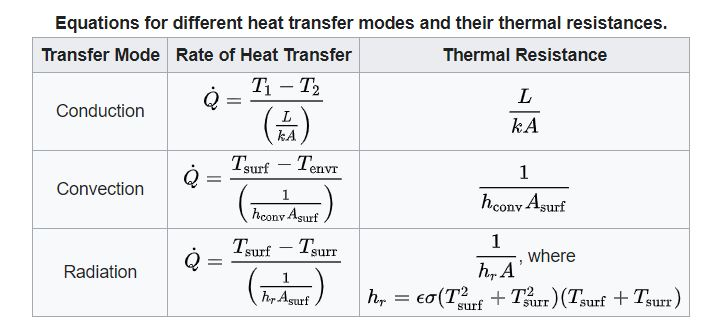
\includegraphics[width=0.8\columnwidth]{Pictures/heat transfer mode.JPG}
	\caption[Short title]{Heat transfer modes\cite{GIGO}}
	\label{table_1}
\end{figure}
\newpage

In \cite{HTTHERMO} and \cite{FUND} the expressions in Fig.\ref{table_1} are derived.
For conduction, the expression for absolute thermal resistance is:  

\begin{equation}
	R = \frac{L}{kA} \qquad \left[ \frac{K}{W} \right]
\end{equation}

\begin{itemize}
    \item $L$ is the distance over which heat transfer takes place, or the thickness of the material $[m]$.
    \item $k$ (also denoted with $\lambda$) is the thermal conductivity of the material. [$\frac{W}{mK}$]. 
    \item $A$ is the conductive surface area  $[m^2]$.
    \item Thermal resistivity is the reciprocal of thermal conductivity and can be expressed as $r =\frac{1}{k}$  in $[\frac{mK}{W}]$

\end{itemize}


For convection and radiation the expression for thermal resistance is: $R = \frac{1}{h \cdot A}$ [$\frac{K}{W}$].

\begin{itemize}
    \item $A$ is the surface area where the heat transfer takes place $[m^2]$.
    \item $h$ is the heat transfer coefficient  [$\frac{W}{m^2K}$]
\end{itemize}


The $R$-value (in Dutch: $R$-waarde or $R_d$-waarde) of a building material \cite{Rvalues_insulation} is the thermal resistance of a square meter surface.
It can be calculated by multiplying the thermal \emph{resistivity} with the thickness of the material in  $m$.
Alternatively it is calculated by dividing the material thickness by the thermal \emph{conductivity} $k$ or $\lambda$.

\begin{equation}
	\text{R-value} = r \cdot L  \qquad \text{or} \qquad  \text{R-value} = \frac{L}{k}  \qquad \text{or} \qquad  
	\text{R-value} = \frac{L}{\lambda}  \qquad \left[m \cdot \frac{m \cdot K}{W} \right] = \left[\frac{m^2 \cdot K}{W}\right] 
\end{equation}


Some typical heat transfer $R$-values are: \cite{OVERALL}: 

\begin{itemize}
	\item Static layer of air, 40 mm thickness (1.57 in)  : R = 0.18 [$\frac{m^2K}{W}$].
	\item Inside heat transfer resistance, horizontal current : R = 0.13 [$\frac{m^2K}{W}$]. 
	\item Outside heat transfer resistance, horizontal current : R = 0.04 [$\frac{m^2K}{W}$].
	\item Inside heat transfer resistance, heat current from down upwards : R = 0.10 [$\frac{m^2K}{W}$].
	\item Outside heat transfer resistance, heat current from above downwards : R = 0.17 [$\frac{m^2K}{W}$].
\end{itemize}


\textbf{Note}: in Dutch building physics, $R$-values with subscripts are used:
\begin{itemize}
	\item $R_d$-waarde is used for the $R$-value of a homogeneous building material. $ R = \frac{L}{\lambda} $
	\item $R_c$-waarde (compound, construction) is used for the $R$-value of a surface consisting of several building materials. $R_c$-waarden are calculated as the surface-area weighted sum of $R_d$-waarden of the building materials. 
	For the simplest roof surface, $R_c$ is a linear combination of the $R$-values of the wooden joists and girders (spanten en gordingen) and the areas in between with a certain insulation material sandwich.
	The $R$-value of the insulation sandwich, in its turn, is the sum of the $R$-values of the materials in the sandwich. From inside out, this sandwich may consist of \textit{e.g.} a 9.5 mm plaster board, a PIR/PUR insulation panel, an air gap and a wooden roof deck. All types of $R$-value have the dimension $ [\frac{m^2 \cdot K}{W}] $.
\end{itemize}

\begin{figure}[H]
	\centering
	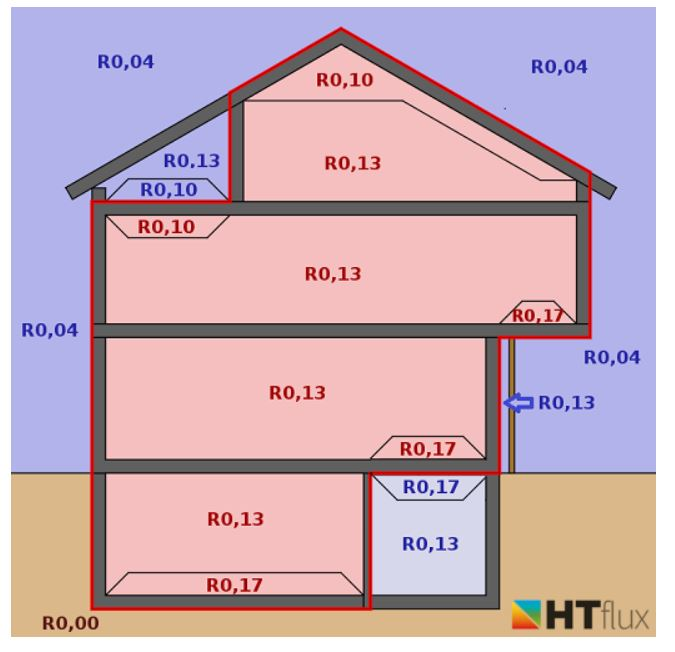
\includegraphics[width=0.8\columnwidth]{Pictures/Overview of heat resistances.JPG}
	\caption[Short title]{An overview of $R$-values for heat transfer \cite{SURFREST}.}
	\label{fig:overview}
\end{figure}


The standard R\textsubscript{c}-values that have been used for facades, roof and floor until 2020 are summarized in Fig.\ref{fig:Rcvalues}:

\begin{figure}[H]
	\centering
	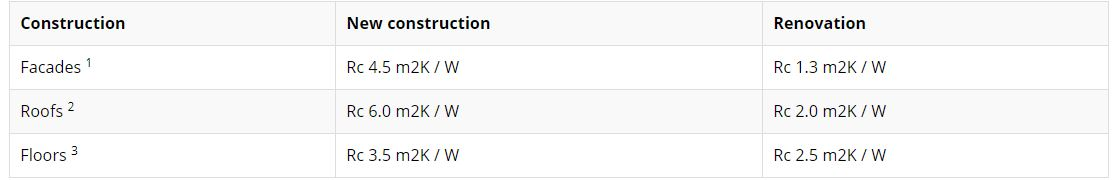
\includegraphics[width=1.0\columnwidth]{Pictures/Rc_values_2020.JPG}
	\caption[Short title]{R\textsubscript{c} Values \cite{ISOL}}
	\label{fig:Rcvalues}
\end{figure}

New standard values will be used from 1-1-2021, since the building standard NEN 1068 will be replaced by the NTA 8800 standard. The old and new situation is described in "EnergieVademecum Energiebewust ontwerpen van nieuwbouwwoningen", Hoofdstuk 5: Thermische isolatie, thermische bruggen en luchtdichtheid.
\cite{ISSO}.

\begin{figure}[H]
	\centering
	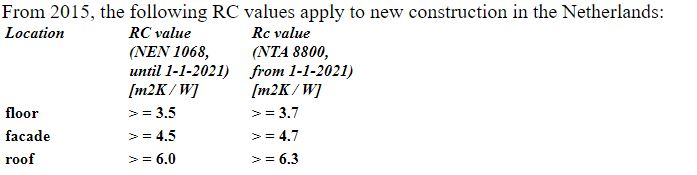
\includegraphics[width=1.0\columnwidth]{Pictures/Rc_values_2021.JPG}
	\caption[Short title]{R\textsubscript{c} Values \cite{RVALUE}}
	\label{fig:newRc}
\end{figure}

The values used for different types of houses such as: row houses, detached houses and apartments can be found in the document "Voorbeeldwoningen 2011" \cite{VOORBEELD}. An example with values for a common type of row house, built in the period from 1975 to 1991 is shown in Fig. \ref{row_house}:


\begin{figure}[H]
	\centering
	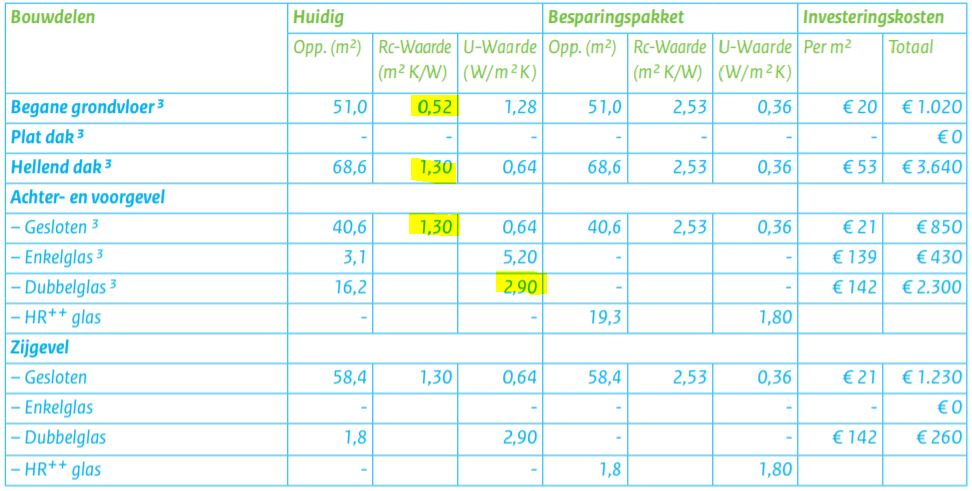
\includegraphics[width=0.8\columnwidth]{Pictures/row_house_1975-1991.JPG}
	\caption[Short title]{R\textsubscript{c}-values for a row house type built between 1975-1991 \cite{VOORBEELD}}
	\label{row_house}
\end{figure} 
\newpage

\subsection{Dwelling (envelope) model analogous to a 2R-2C network}

The heat flow will be modelled by analogy to an electrical circuit where heat transfer rate is analogous to by current, temperature difference is analogous to potential difference, heat sources are represented by constant current sources, absolute thermal resistances are represented by resistors and \textbf{thermal capacitance} heat capacity ? by capacitors \cite{AbsTR}. Figure \ref{fig:Analogies} summarizes the similar term use in different fields.

\begin{figure}[H]
	\centering
	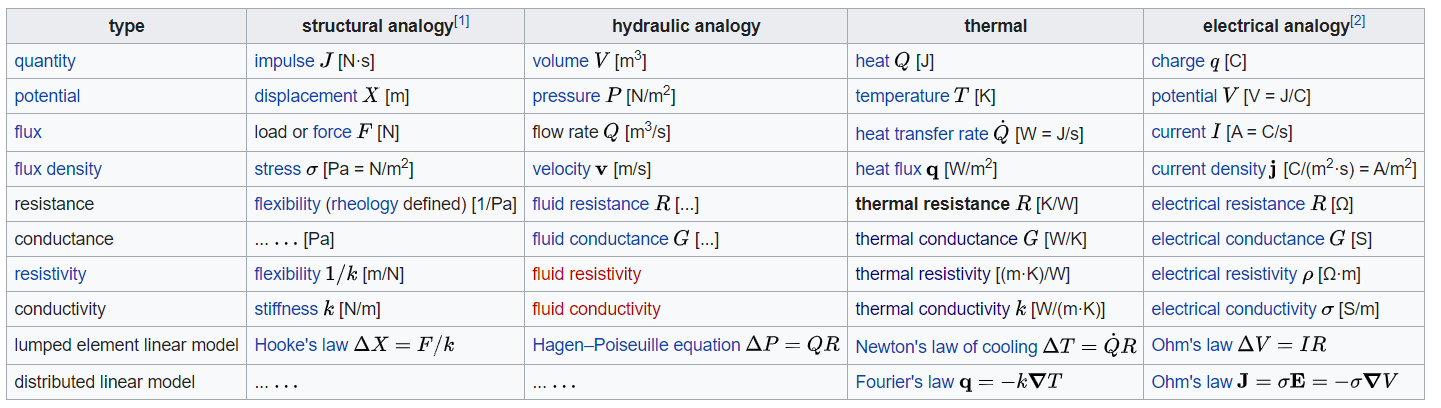
\includegraphics[width=1.0\columnwidth]{Pictures/Analogies.png}
	\caption[Short title]{Table of Analogies  \cite{AbsTR}}
	\label{fig:Analogies}
	\end{figure} 

The 2R-2C house model structure is implemented as described below. The schematic of an envelope house model has been shown in figure  \ref{fig:envelope2R2C} and the equivalent electrical 2R-2C network with components and topology is given in fig  \ref{fig:elec2R2C}.

\begin{figure}[H]
	\centering
	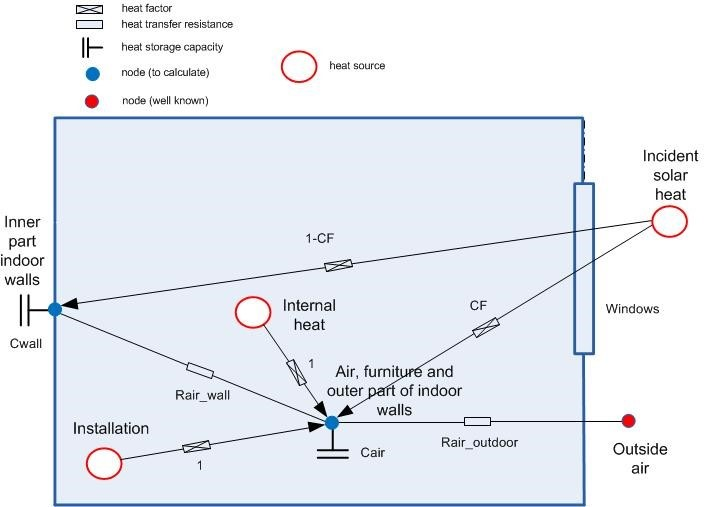
\includegraphics[width=1.0\columnwidth]{Pictures/envelopRC.jpg}
	\caption[Short title]{Schematic of envelope model}
	\label{fig:envelope2R2C}
	\end{figure} 
	

\begin{figure}[H]
	\centering
	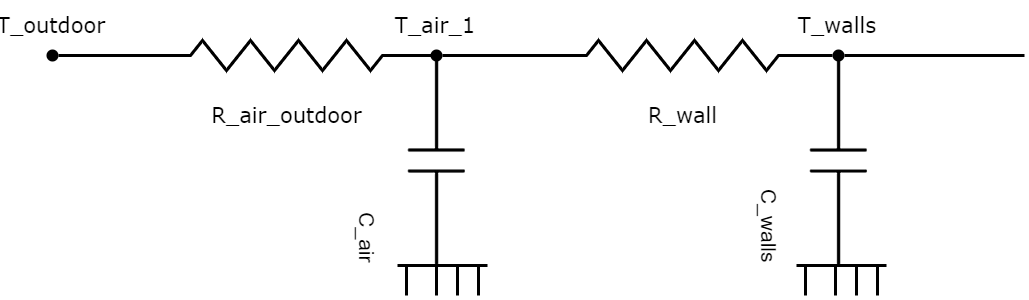
\includegraphics[width=1.0\columnwidth]{Pictures/2R2C_Model.png}
	\caption[Short title]{2R-2C house model}
	\label{fig:elec2R2C}
	\end{figure}
	
The model consists of two heat capacities C\textsubscript{air, indoor} and C\textsubscript{wall} and two resistances R\textsubscript{wall} and R\textsubscript{air, outdoor}. The incident solar energy is divided between C\textsubscript{wall} and C\textsubscript{air} through the convection factor CF. It is assumed that both internal heat (lighting, occupancy and electric devices) and supplied heat (installation) initially heat up the indoor air. In Fig. \ref{fig:envelope2R2C}, they are fully released at the T\textsubscript{air} node. 

 It is also assumed that furniture and the \textbf{surface part} of the walls have the same temperature as the air \textbf{and the wall mass is divided between the air and wall mass}. Thus, the heat capacity of the air node consists of the air heat capacity, furniture heat capacity and the heat capacity \textbf{of a part of the walls}. \textbf{Appendix A} presents the coefficients in the dwelling model. In the resistance R\textsubscript{air, outdoor} the influence of heat transmission through the outdoor walls and natural ventilation is considered. 
 
For the air and wall nodes the following power balances can be set up: 

\begin{equation}
C_{air}\frac{dT_{air}}{dt}=\frac{T_{outdoor}-T_{air}}{R_{air_{\_}outdoor}} + \frac{T_{wall}-T_{air}}{R_{air_{\_}wall}} + \dot{Q}_{inst} + \dot{Q}_{internal} + CF\cdot\dot{Q}_{solar}
\end{equation}

\begin{equation}
C_{wall}\frac{dT_{wall}}{dt}=\frac{T_{air}-T_{wall}}{R_{air_{\_}wall}} + (1-CF)\cdot\dot{Q}_{solar}
\end{equation}


 \begin{itemize}
      \item $CF$: convection factor (solar radiation): the convection factor is the part of the solar radiation that enters the room and is released directly convectively into the room.
      \item $\dot{Q}_{inst}$: delivered heat from heating system (radiator) [W].
      \item $\dot{Q}_{inernal}$: internal heat [W].
      \item $\dot{Q}_{solar}$: heat from solar irradiation [W].
      \item $T_{air}$: indoor air temperature $^o$C.
      \item $T_{outdoor}$: outdoor temperature $^o$C.
      \item $T_{wall}$: wall temperature $^o$C.
      \item $R_{air_{\_}wall}$: walls surface resistance [$\frac{K}{W}$].
      \item $R_{air_{\_}outdoor}$: outdoor surface resistance [$\frac{K}{W}$].
      \item $C_{air}$: air thermal capacitance (heat capacity) [$\frac{J}{K}$]\cite{Thermalmass}.
      \item $C_{wall}$: wall thermal capacitance (heat capacity) [$\frac{J}{K}$]\cite{Thermalmass}.
    \end{itemize}

\newpage   

Total heat transfer of solar irradiation through the glass windows. 
\begin{equation}
\dot{Q}_{solar}=g.\sum(A_{glass}.\dot{q}_{solar})
\end{equation}

\begin{itemize}
    \item $\dot{q}_{solar}$: solar radiation on the outdoor walls [$\frac{W}{m^2}$]. 
    \item g: g value of the glass (ZTA in dutch) [0..1]\cite{zontoetreding}
    \item A: glass surface [$m^2$].
\end{itemize}

%7.6.6.1.2 Ramen met niet-verstrooiende beglazing NTA8800
%https://help.dgmr.nl/bink9/zontoetredingsfactor-zta.html
%https://www.joostdevree.nl/shtmls/zta.shtml
%ISSO-Handboek Zonnestraling: 5.5.1 en 5.2


\newpage


% \section{Dwelling (envelope) model analogous to a 2R-2C network}

The 2R-2C house model structure is implemented as described below:
	
\begin{figure}[H]
	\centering
	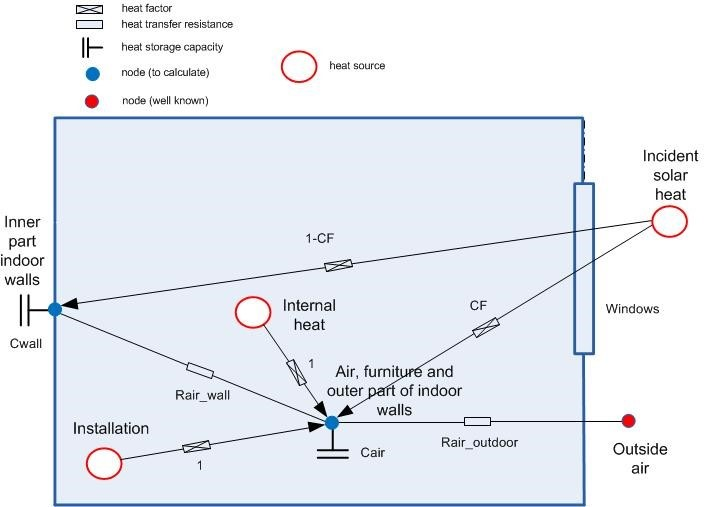
\includegraphics[width=1.0\columnwidth]{Pictures/envelopRC.jpg}
	\caption[Short title]{Schematic of envelope model}
	\label{fig:envelope2R2C}
	\end{figure} 
	
The equivalent electrical 2R-2C network with components and topology is given in Fig. \ref{fig:elec2R2C}.

\begin{figure}[H]
	\centering
	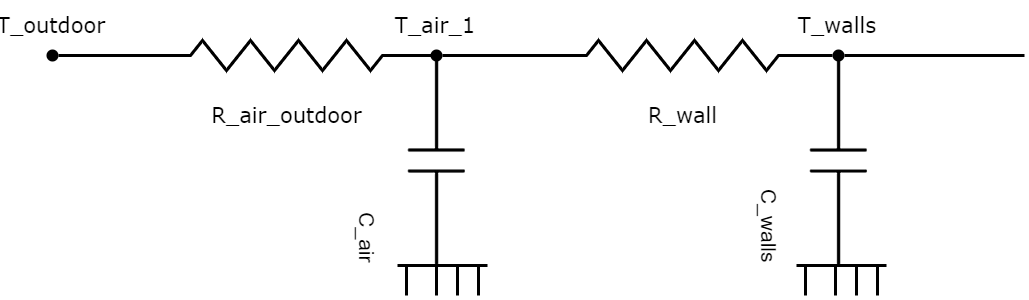
\includegraphics[width=1.0\columnwidth]{Pictures/2R2C_Model.png}
	\caption[Short title]{2R-2C house model}
	\label{fig:elec2R2C}
	\end{figure}
	
The model consists of two capacitances C\textsubscript{air, indoor} and C\textsubscript{wall} and two resistances R\textsubscript{wall} and R\textsubscript{air, outdoor}. The incident solar energy is divided between C\textsubscript{wall} and C\textsubscript{air} through the convection factor CF. It is assumed that both internal heat (lighting, occupancy and electric devices) and supplied heat (installation) initially heat up the indoor air. In Fig. \ref{fig:elec2R2C}, they are fully released at the T\textsubscript{air} node. 

 It is also assumed that furniture and the surface part of the walls have the same temperature as the air and the wall mass is divided between the air and wall mass. Thus, the capacity of the air node consists of the air capacity, furniture capacity and capacity of a part of the walls. \textbf{Appendix A} presents the coefficients in the dwelling model. In the resistance R\textsubscript{air, outdoor} the influence of heat transmission through the outdoor walls and natural ventilation is considered. 
 
For the air and wall nodes the following energy balances can be set up: 

\begin{equation}
C_{air}\frac{dT_{air}}{dt}=\frac{T_{outdoor}-T_{air}}{R_{air_{\_}outdoor}} + \frac{T_{wall}-T_{air}}{R_{air_{\_}wall}} + \dot{Q}_{inst} + \dot{Q}_{internal} + CF\cdot\dot{Q}_{solar}
\end{equation}

\begin{equation}
C_{wall}\frac{dT_{wall}}{dt}=\frac{T_{air}-T_{wall}}{R_{air_{\_}wall}} + (1-CF)\cdot\dot{Q}_{solar}
\end{equation}

 \begin{itemize}
      \item CF: Convection factor (solar radiation): the convection factor is the part of the solar radiation that enters the room and is released directly convectively into the room
      \item $\dot{Q}_{inst}$: delivered heat from heating system (radiator) [W].
      \item $\dot{Q}_{solar}$: heat from solar irradiation [W].
      \item $T_{air}$: indoor air temperature $^o$C.
      \item $T_{outdoor}$: outdoor temperature $^o$C.
      \item $T_{wall}$: wall temperature $^o$C.
      \item $R_{air_{\_}wall}$: walls surface resistance [$\frac{K}{W}$].
      \item $R_{air_{\_}outdoor}$: outdoor surface resistance [$\frac{K}{W}$].
      \item $C_{air}$: air capacity [$\frac{J}{K}$].
      \item $C_{wall}$: wall capacity [$\frac{J}{K}$].
    \end{itemize}
    

Total heat transfer of solar irradiation through the glass windows. 
\begin{equation}
Q_{solar}=g.\sum(A_{glass}.q_{solar})
\end{equation}

\begin{itemize}
    \item $q_{solar}$: solar radiation on the outdoor walls [$\frac{W}{m^2}$]. 
    \item g: g value of the glass (ZTA in dutch) [0..1]\cite{zontoetreding}
    \item A: glass surface [$m^2$].
\end{itemize}

%7.6.6.1.2 Ramen met niet-verstrooiende beglazing NTA8800
%https://help.dgmr.nl/bink9/zontoetredingsfactor-zta.html
%https://www.joostdevree.nl/shtmls/zta.shtml
%ISSO-Handboek Zonnestraling: 5.5.1 en 5.2

\newpage

\section{Simulink model user guideline}

The dwelling model has been fist developed in Matlab/Simulink and convert to Python later on. In the Simulink model it is possible to define the dwelling characteristics, the dwelling use data and the climate data. With some of this information the model resistances and capacities are built on a Matlab script. The resistances and capacities values are used during the year energy simulation. 
In sections \ref{Dewellinginfo} to \ref{climatedata} the information provided to make the simulation is presented.

\subsection{Dwelling characteristics information}
\label{Dewellinginfo}
	
The dwelling characteristics taken into account in order to define the model resistances and capacities are presented in figure \ref{figure: Dwelling characteristic}. The ventilation rate n in ach (air changes per hour) is based on a mechanical ventilation rate of 150 m3/h for kitchen, toilet and bathroom) by regulations.

\begin{figure}[H]
	\centering
	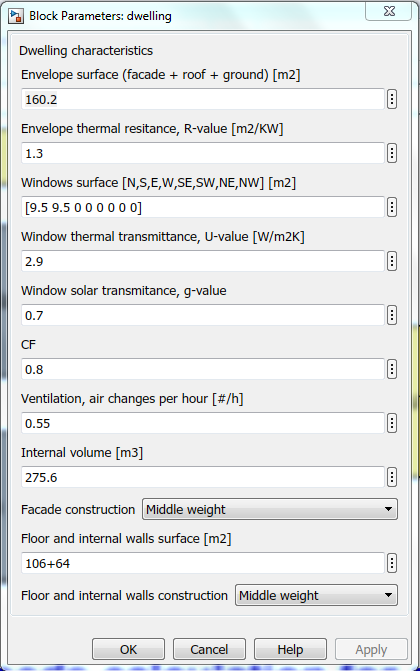
\includegraphics[width=0.8\columnwidth]{Pictures/dwelling characteristic model information.png}
	\caption[Short title]{Dwelling characteristic model information}
	\label{figure: Dwelling characteristic}
\end{figure}
\newpage
\subsection{Dwelling use data}
\label{Dwelling use data}

The dwelling use data define the schedule to be used to calculate the dwelling internal heat and the thermostat set-points. The thermostat signal is communicated to the heat pump model. The information use to define the dwelling use is presented in figure \ref{figure:Dwelling info}


\begin{figure}[H]
	\centering
	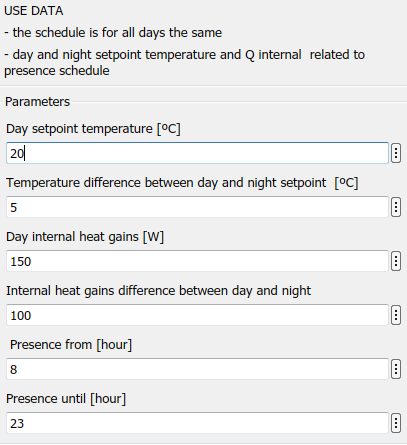
\includegraphics[width=0.8\columnwidth]{Pictures/Dwelling use model information.png}
	\caption[Short title]{Dwelling use model information}
	\label{figure:Dwelling info}
\end{figure}
\newpage
\subsection{Climate data}
\label{climatedata}
The hourly data about the outdoor temperature and the solar radiation is extracted from the NEN5060:2018 norm. This norm defines a typical meteorological year using the Finkelstein-Schafer statistical method with the climate data of 20 years period (1996-2015). The meteorological data used by the norm is updated once every 5 years.  

The typical meteorological year data is the one to be used when calculating the typical energy use of the heating installation. The NEN norm offers also three other hourly climate data sets, each one with a different perceptual deviation from the typical meteorological year: 1\%, 3\% and 5\%. These data sets are to be used when analysing the response of the heating installation under more extreme climate conditions. This is usually done for design installation purposes. The total energy use calculated with these other data sets will not give a reliable value for calculating the typical energy use.  In figure \ref{figure Climate data selection} it is shown that is it possible to choose between the four different NEN climate data sets. 

\begin{figure}[H]
	\centering
	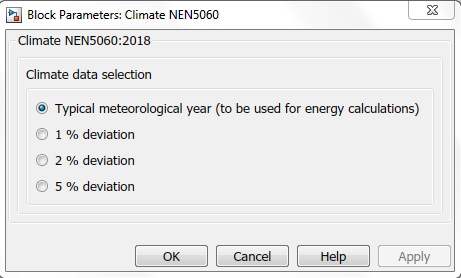
\includegraphics[width=0.8\columnwidth]{Pictures/climate data selection.png}
	\caption[Short title]{Climate data selection}
	\label{figure Climate data selection}
\end{figure}

In a pre-process the global incident radiant is calculated for North, South, East, West, North-West, North-East, South-West and South-East orientations of the façade in Matlab. The model from Perez is applied for the exchange. In this model the irradiation is split into a direct and diffuse terms.
\newpage


\section{Simulation, results and verification}

\subsection{Simulation}
In order to calculate the inside temperature of the house the model considers five heat flow. 

\begin{itemize}
    \item Transmission
    \item Ventilation
    \item Solar Gains
    \item Internal Heat Gains
    \item Heating/Cooling
\end{itemize}

The model also considers the mass of the air inside the house and the mass of the walls.  
House characteristics data.

The document Voorbeeldwoningen 2011 Bestaande bouw published by Agentschap NL \cite{VOORBEELD} will be used as a reference to determine the house characteristics. The document makes a classification of the house stock per construction type (7) and year of construction (4 time periods).  

\textbf{Construction type.}
\begin{itemize}
    \item Detached house (vrijstaande woning)
    \item Semi-detached house (2 onder 1 kap woning)
    \item Terraced house (rijwoning)
    \item Apartment block own access (maisonnettewoning)
    \item Apartment horizontal shared access (galerijwoning)
    \item Apartment block vertical shared access (portiekwoning)
    \item Apartment block in general (flatwoningen (overig))
    
\end{itemize}
\textbf{Year of construction.}
\begin{itemize}
    \item Build before 1964
    \item Build between 1965 and 1974
    \item Build between 1975 and 1991
    \item 	Build between 1992 and 2005
\end{itemize}

For the first model, the data of a detached house building build between 1975 and 1991 has been used. 
The energy consumption sum presented in the report as the first validation mechanism for this model. In the following model development, we should look for the possibility to validate the model with the use of real data.

\textbf{Climate data.}\\
NEN 5060:2008 and 2018 nl (Hygrothermische eigenschappen van gebouwen -Referentieklimaatgegevens), will be used as the climate data for the simulations.

\textbf{Internal heat gains data.}\\
There is no reference document about the internal heat gains for dwelling in the Netherlands. We can consider that there are two people living in the house with an average working schedule.
Control mechanism
The heating will be controlled by a thermostat. The indoor temperature of the house is based on recommendation given on the ISSO publication Kleintje Binnenklimaat. The indoor temperature should be maintained at a minimum of 20 degrees. 
We could consider taking cooling into account. 


\subsection{Results}
To test the model, we have used the data from the document Voorbeeldwoningen 2011 Bestaande bouw published by Agentschap NL \cite{VOORBEELD}. We have run the model for a detached house building build between 1975 and 1991 and for row house building build between 1975 and 1991.For the detached house the model calculates a sum of the yearly energy needs of 10545 kWh. The document Voorbeeldwoningen 2011 gives a calculated energy use for heating and hot water of 1542 m3 gas. The average gas consumption of hot tap water on a Dutch household is 300 m3gas. We assume a combustion (under) value ho=35.2 MJ/m3 gas. Taking into consideration a heating system efficiency of 0.9, the energy need is 10843 kWh. 


\begin{equation}
\frac{(1542-300) \cdot 35200}{3600\cdot 0.9}= 10843[KWh] 
\end{equation}


For the row house the model calculates a sum of the yearly energy needs of 19776 kWh. The sidewalls have been considered as adiabatic walls. The document Voorbeeldwoningen 2011 gives a calculated energy use for heating and hot water of 2616 m3 gas. The average gas consumption of hot tap water on a Dutch household is 300 m3gas. Taking into consideration a heating system efficiency of 0.9, the energy need is 20219 kWh. 

\begin{equation}
\frac{(2616-300) \cdot 35200}{3600\cdot 0.9}= 20129[KWh] 
\end{equation}

The results give an indication that the model is on the right result range for detached and row house.

The plot on figure \ref{fig:Simulationresults}, show the comparison of simulation results and annual heating consumption in Voorbeeldwoningen 2011 \cite{VOORBEELD}. More results can be found in Appendix B

\begin{figure}[H]
	\centering
	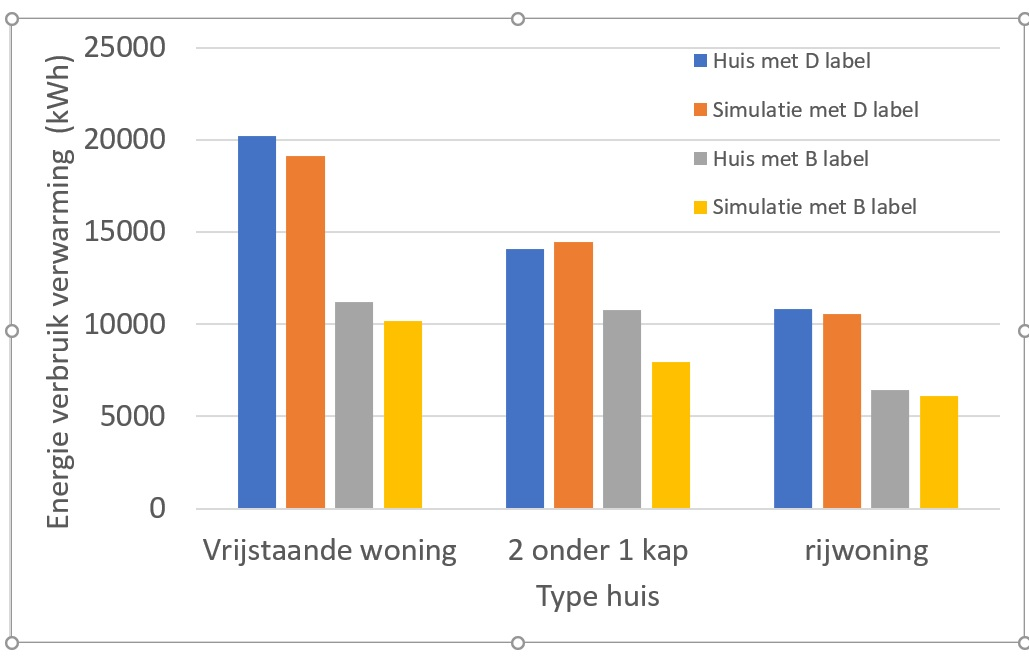
\includegraphics[width=1.0\columnwidth]{Pictures/Simulation results.jpg}
	\caption[Short title]{Simulation versus energy usage}
	\label{fig:Simulationresults}
	\end{figure}
\newpage

The graph in figure \ref{fig:heatingvstemp} shows the yearly heating demand needed for difference outdoor temperature.
It is clearly show the typical whether condition in the Netherlands where most of the energy use for heating happen at temperature range from 4 to 8 degree $^oC$.

\begin{figure}[H]
	\centering
	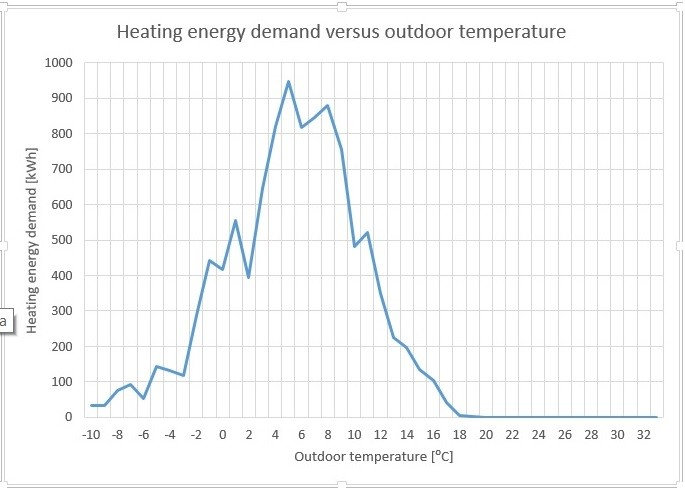
\includegraphics[width=1.0\columnwidth]{Pictures/Yearheatingdemand.jpg}
	\caption[Short title]{Simulation versus energy usage}
	\label{fig:heatingvstemp}
	\end{figure}
	
In order to get an estimation of the minimum heating power capacity needed to maintain a specific indoor temperature for the whole year the model thermostat has been set at a constant temperature day and night.
Minimum heating power capacity needed to maintain a specific indoor temperature has been shown in table 1.

\begin{table}[H]
    \centering
    \begin{tabular}{|c|c|}
    \hline
    Indoor temperature $[^oC]$  & Minimum heating powercapacity $[W]$ \\
    
    \hline
     18     &  6041 \\
     
     \hline
     19     &  6335 \\
     
     \hline
     20     &  6474 \\
     
     \hline
     21     &  6704 \\
     
     \hline
     22     &  6972 \\
     
     \hline
     23     &  7144 \\
     
     \hline
     24     &  7366 \\
     
    \hline

    \end{tabular}
    \caption{Minimum heating powercapacity}
    \label{tab:Minimumheat}
\end{table}
 
\newpage

\section{Data driven model and prediction}

This section will present a method for heat demand prediction base on machine learning technique.

%\subsection{Parameters estimation.}

\subsection{LSTM model.}

Long short term memory model or LSTM is a very special kind of recurrent neural network which used in application such as speech recognition, language modeling, translation, text generation ..etc. Christopher Olah gave an excellent explanation on LSTM model and how does it work in her blog. \cite{LSTM}.The structure of LSTM model can be seen in figure \ref{fig:LSTM}.

There are many types of LSTM models that can be used for each specific type of time series forecasting problem.These are problems comprised of series of observations and a model is required to learn from the series of past observations to predict the next value in the sequence.

\begin{figure}[H]
	\centering
	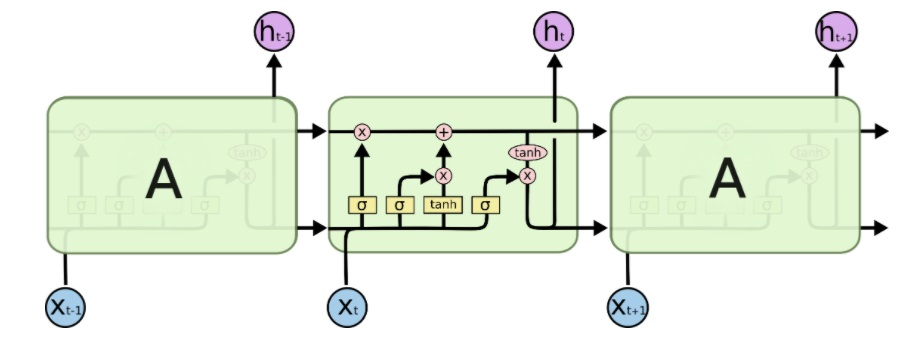
\includegraphics[width=1.0\columnwidth]{Pictures/LSTM strcuture.jpg}
	\caption[Short title]{LSTM model strcuture}
	\label{fig:LSTM}
	\end{figure}


In this study an multivariate LSTM model has been developed using Pytorch (Facebook famous machine learning open source library) for heat demand prediction inside a dwelling. The goal of this study is showing a proof of concept on how the model can learn the dynamic behaviour of different house.

The data has been generated from house simulation model and NEN-2018 weather data file. The first 70\% is used for training and  30\% left for validation.

\subsection{Model Prediction}

The model can predict the next hours heat demand base on the previous 12 hours pass inputs data. The inputs data consist of: 

\begin{itemize}
    \item $T_{a}$: Ambient temperature $[^o C]$.
    \item $SP$   : The temperature set point profile$[^o C]$. 
    \item $\dot{Q}_{Solar}$: Heat generated from solar irradiation $[W/m^2]$.
    \item $\dot{Q}_{inernal}$: Internal heat gain from the present people and furniture inside the house [W].
    \item $\dot{Q}_{inst}$: delivered heat from heating system (radiator) [W].
\end{itemize}

The simulation result in figure \ref{fig:heat demand prediction} and \ref{fig:50 days heat demand prediction} show that the model give a good prediction for an hour figure \ref{fig:heat demand prediction} and multiple hours figure \ref{fig:50 days heat demand prediction} heat demand.

\begin{figure}[H]
	\centering
	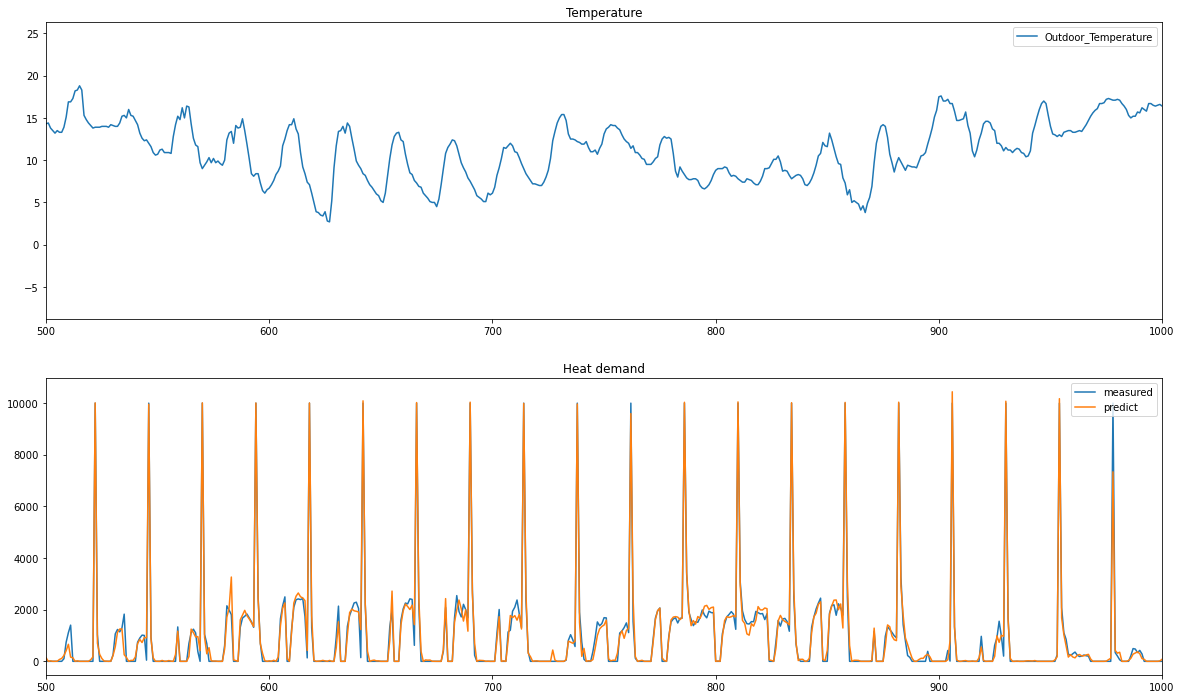
\includegraphics[width=1.0\columnwidth]{Pictures/house heat demand prediction zoom.png}
	\caption[Short title]{Heat demand prediction for light weight construction.}
	\label{fig:heat demand prediction}
	\end{figure}

The simulation result in figure \ref{fig:heat demand prediction} shows that the model give a good prediction for the next hour heat demand needed.

\begin{figure}[H]
	\centering
	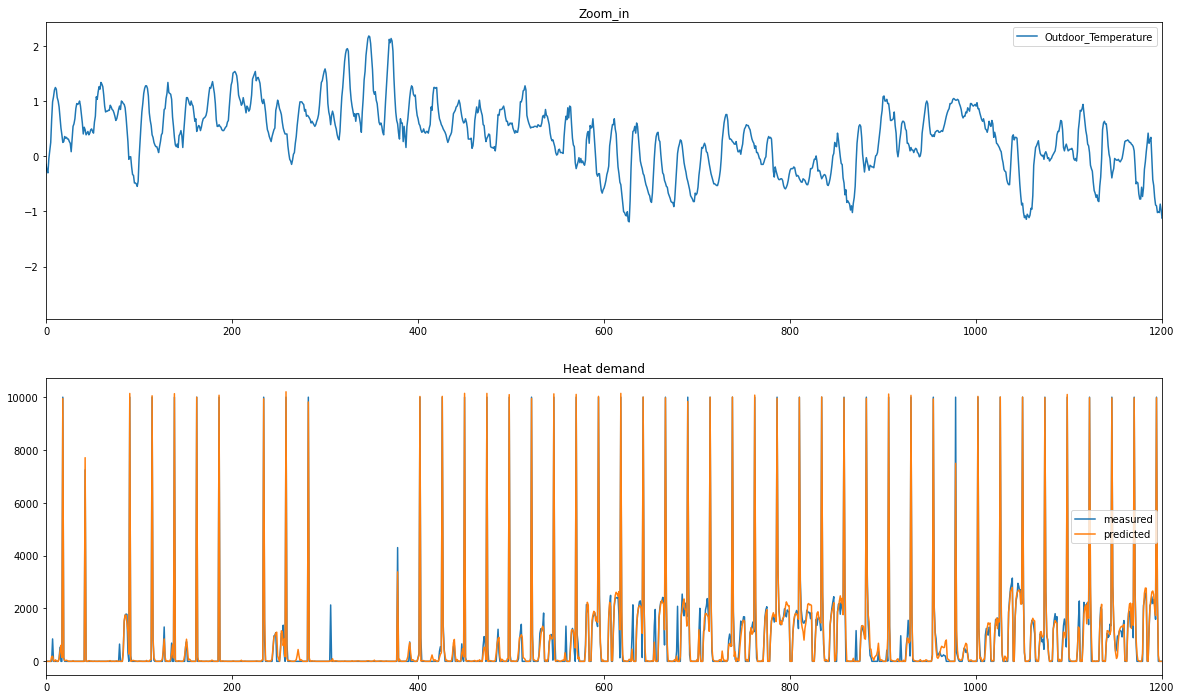
\includegraphics[width=1.0\columnwidth]{Pictures/50days_heat_demand_prediction.png}
	\caption[Short title]{50 days heat demand prediction.}
	\label{fig:50 days heat demand prediction}
	\end{figure}


The prediction above has based on the assumption that all the parameters such as $T_{a}$, $SP$, $\dot{Q}_{Solar}$, $\dot{Q}_{inernal}$ and $\dot{Q}_{inst}$ for the pass and current time are well known. The result show that the prediction accuracy reduce if solar power and internal heat gain at the current time are not known (in this simulation solar power and internal heat gain are set to zero) figure \ref{fig:hour prediction with uncertainties}.

\begin{figure}[H]
	\centering
	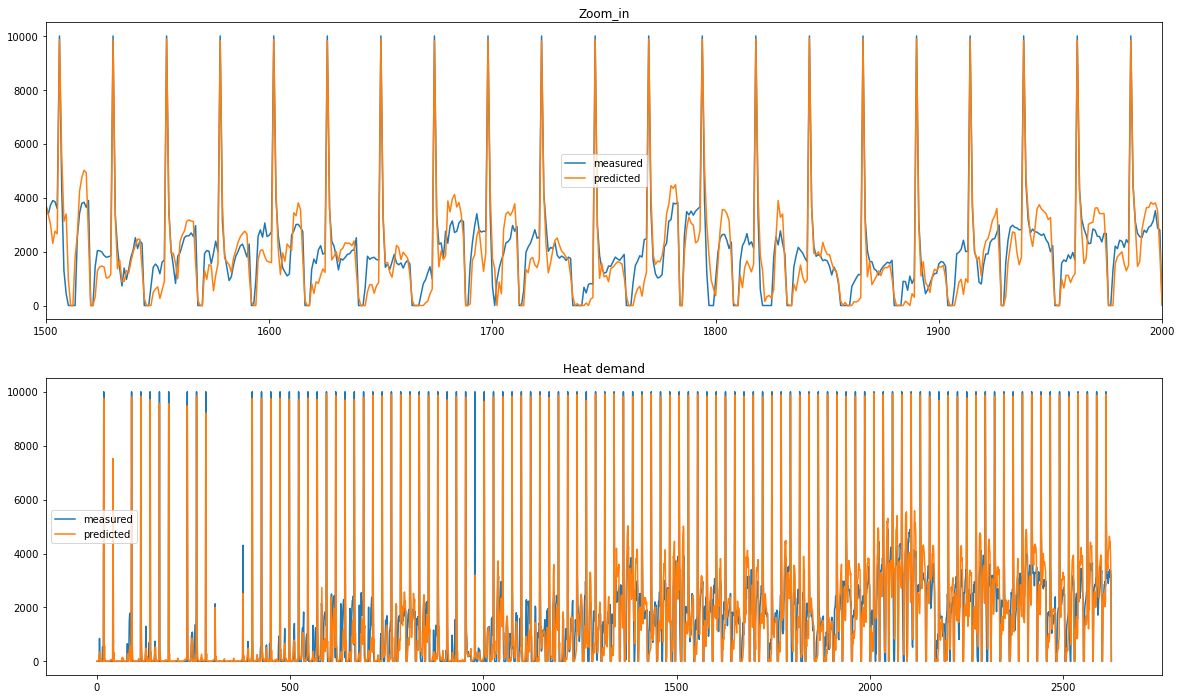
\includegraphics[width=1.0\columnwidth]{Pictures/1hour_heatdemand_with_uncertainties.png}
	\caption[Short title]{1 hour heat demand prediction with uncertainties}
	\label{fig:hour prediction with uncertainties}
	\end{figure}
	
In summary, to be able to have a good heat demand prediction, the model need to be trained with a good data sources which can represent the dynamic behaviour of the house in all scenarios. The more data in different situations use for the training step the more accurate the prediction is.   

\newpage

%\section{Heat demand prediction model using machine learning.}

This chapter will summarize report of the minor project students from big data module.
There are 2 data sets had been used. One of these data sets was delivered by a member of HAN. It contains the weekly heat production of a house with a heat pump and a gas heating. This data set would provide the information about the heat demand, the output of the model. The other data set used was the weather data of the closest weather station (Instituut, 2019). This data set would provide the inputs to the model, consisting of the average weekly temperature, the average weekly wind speed, the average weekly sunshine duration the overall sum of sunshine duration, the average hourly precipitation and the sum of precipitation per week. This data was gained from hourly values provided by the Dutch weather service.\\
The heat production data was manually cleaned to get rid of outliers, measurement errors and other unwanted values. Dimensions of each column were checked, gaps filled and intervals between data checked for uniformity. As the heat production was given as an accumulative sum, the heat production per week needed to be extracted.
The data was split to 70${\%}$ for training and 30${\%}$ for testing.
As the NN was doing classification in the assignment, the evaluation had to be changed as well. New error metrics for this prediction model had to be established. Mean absolute Error, mean absolute relative error and mean absolute percentage error are a few to name.

\subsection{Neural Network MATLAB toolbox.}

The NN MATLAB toolbox for neural fitting was applied to the data. This toolbox applies a 2-layer feed-forward network with sigmoid hidden neurons and linear output neurons (figures \ref{fig:NNMatlb}). 

\begin{figure}[H]
	\centering
	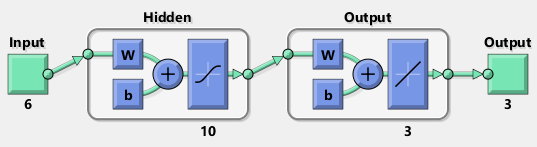
\includegraphics[width=1.0\columnwidth]{Pictures/NN matlab.png}
	\caption[Short title]{NN as used by the neural fitting toolbox}
	\label{fig:NNMatlb}
	\end{figure}

This network is then fed with the $x_{train}$ and $y_{train}$ previously generated for the manual implementation of the NN (figure \ref{fig:NNinput}). 

\begin{figure}[H]
	\centering
	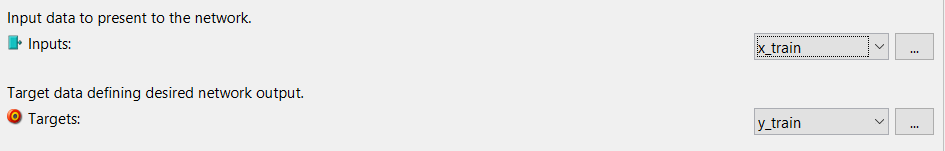
\includegraphics[width=1.0\columnwidth]{Pictures/Input to NN.png}
	\caption[Short title]{Input to NN}
	\label{fig:NNinput}
	\end{figure}

The training data set is then split up into training- test- and validation- set (figure \ref{fig:Trainingvs}). This splitting cannot be reduced to zero. As it is a toolbox function, the validation and test data set were part of the overall training algorithm, so the values were not changed. This data splitting is unconnected to the initial splitting between test and validation set. Here the training data set is internally split up by the toolbox.

\begin{figure}[H]
	\centering
	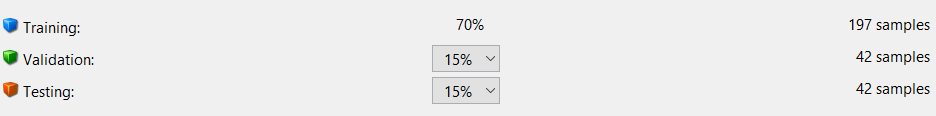
\includegraphics[width=1.0\columnwidth]{Pictures/Training data vs Validation and Testing data ratio.png}
	\caption[Short title]{Training data vs Validation and Testing data ratio}
	\label{fig:Trainingvs}
	\end{figure}

For the hidden layer 10 neurons are chosen.

From the validation performance (figure \ref{fig:Validation Performance}), it can be clearly seen, that the NN is being trained quickly. By the validation performance it is determined, that at epoch 17 the NN delivers best performance so training can be stopped.

\begin{figure}[H]
	\centering
	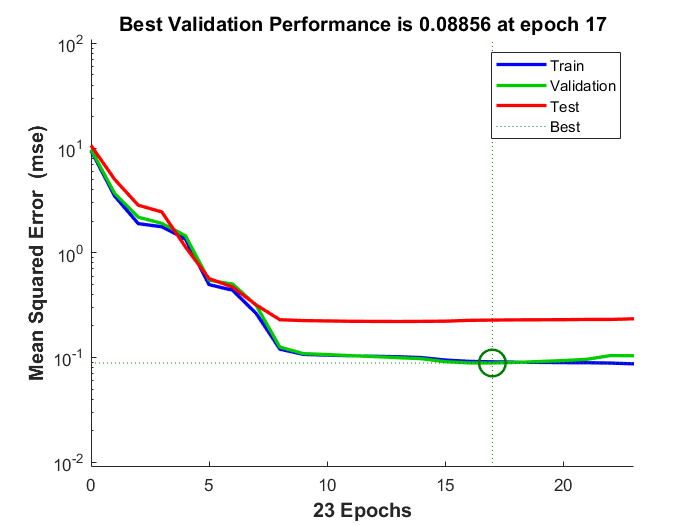
\includegraphics[width=1.0\columnwidth]{Pictures/Validation Performance.png}
	\caption[Short title]{Validation Performance}
	\label{fig:Validation Performance}
	\end{figure}
	
The MSE (mean squared error) can be found in the table \ref{tab:Minimumheat}.

\begin{table}[H]
    \centering
    \begin{tabular}{|c|c|c|}
    \hline
    MSE (norm) & Training Data & Test data \\
    
    \hline
     Heat Pump     &  0.144817 & 0.593376\\
     
     \hline
     Gas           &  0.044751 & 0.218106\\
     
     \hline
     Combine       &  0.136688   & 0.586856\\
    \hline


    \end{tabular}
    \caption{Minimum heating powercapacity}
    \label{tab:Minimumheat}
\end{table}

\subsection{Regression MATLAB toolbox}

The regression SVM toolbox in MATLAB was employed. Using the regression model through SVM  (Gaussian kernel) function, the root mean square error (RMSE) is very small and so are the other error metrics.  A 5-fold cross validation is used to validate the model (figure \ref{fig:k-fold cross validation}).\\
Cross validation is also called a rotation estimation. It’s very easy to see how accurately the predictive model will perform in practical settings. The data is divided into 5 portions of test data sets and training data sets for each iteration. The same test set is not used for all iterations. This testing is just an internal metric of the toolbox and can be seen as part of the training algorithm. It is independent of the initial splitting into test and training data. The cross validation is purely run on the training data. This cross validation is part of the toolbox and can’t be removed.


\begin{figure}[H]
	\centering
	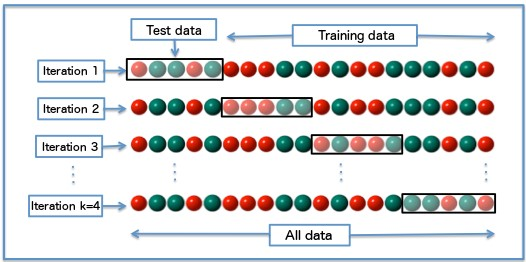
\includegraphics[width=1.0\columnwidth]{Pictures/k-fold cross validation.jpg}
	\caption[Short title]{k-fold cross validation}
	\label{fig:k-fold cross validation}
	\end{figure}
	
The MSE is shown in the table \ref{tab:Minimumheatpower}.

\begin{table}[H]
    \centering
    \begin{tabular}{|c|c|c|}
    \hline
    MSE (norm) & Training Data & Test data \\
    
    \hline
     Heat Pump     &  0.178197 & 0.238478\\
     
     \hline
     Gas           &  0.060874 & 	0.249772\\
     
     \hline
     Combine       &  0.167937   & 0.245215\\
    \hline


    \end{tabular}
    \caption{Minimum heating powercapacity}
    \label{tab:Minimumheatpower}
\end{table}

In the figure \ref{fig:Predicvsactual_temp}, the graph corresponds to the actual heat production and the predicted heat production as given by the toolbox. It can be seen here that there is a good correlation between the output (heat demand) and the temperature (x-axis, $column_{1}$).

\begin{figure}[H]
	\centering
	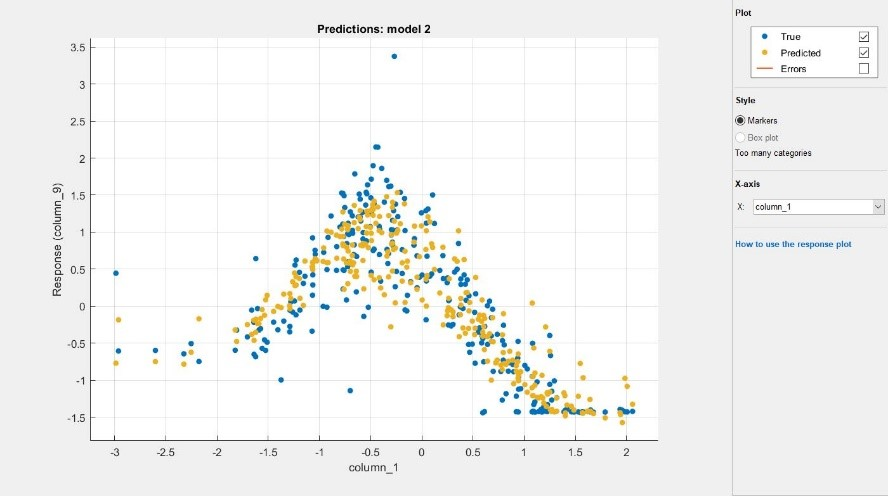
\includegraphics[width=1.0\columnwidth]{Pictures/predicvsheardemand temp.jpg}
	\caption[Short title]{Predicted vs actual heat demand based on temperature}
	\label{fig:Predicvsactual_temp}
	\end{figure}
	
From the simulation results it could be seen that the data gives enough information for prediction. An improvement on the data set would provide better results with any prediction method.
The SVM with the regression toolbox can find a correlation in the data, especially with the temperature input. The MSE for the SVM are even better than the ones of the neural network generated with the toolbox. Also, the MSE on the test data is best for the SVM generated with the regression toolbox. Although it needs training for each output individually, the SVM gives the best predictions.

\newpage
	
	


% \chapter{2 Zones house model 7R4C network}

The 4R-7C house model structure is implemented as described below:
	
\begin{figure}[H]
	\centering
	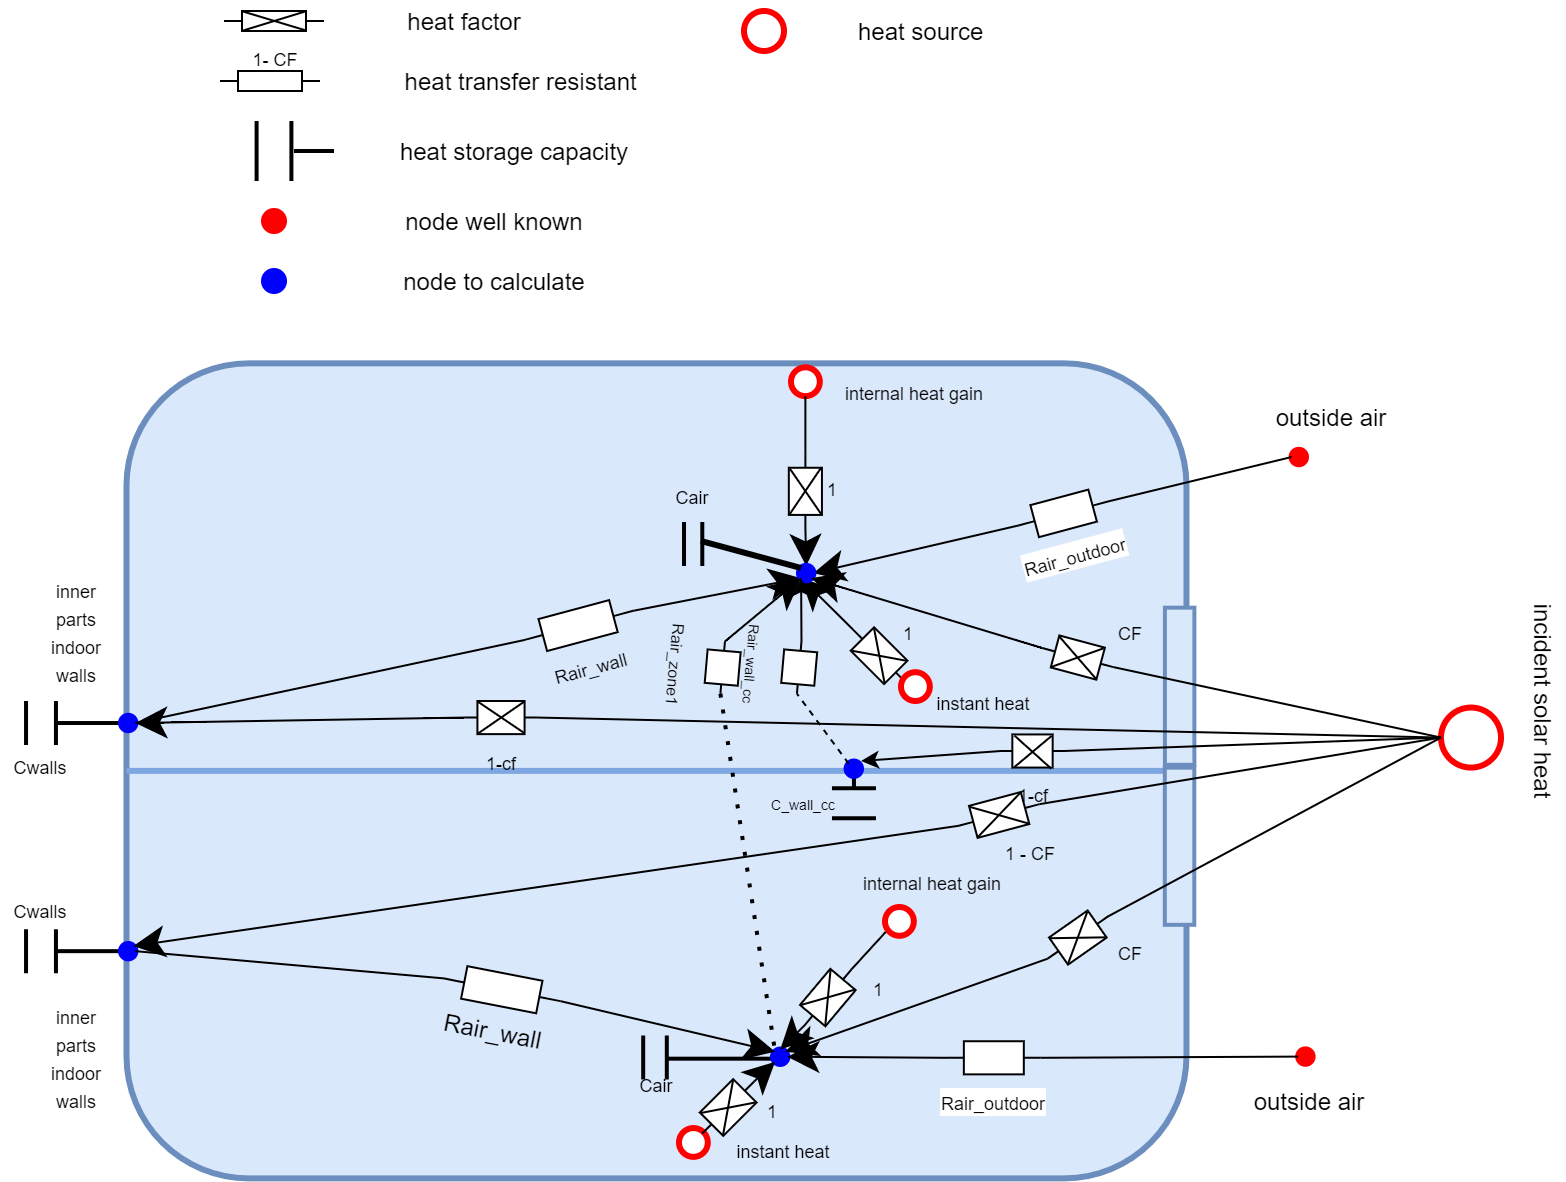
\includegraphics[width=1.0\columnwidth]{Pictures/House_electrical_circuits overview.png}
	\caption[Short title]{Schematic of a 2 zones house model}
	\label{fig:schema7R4C}
	\end{figure} 
	
The equivalent electrical 7R-4C network with components and topology is given in Fig. \ref{fig:elec7R4C}.

\begin{figure}[H]
	\centering
	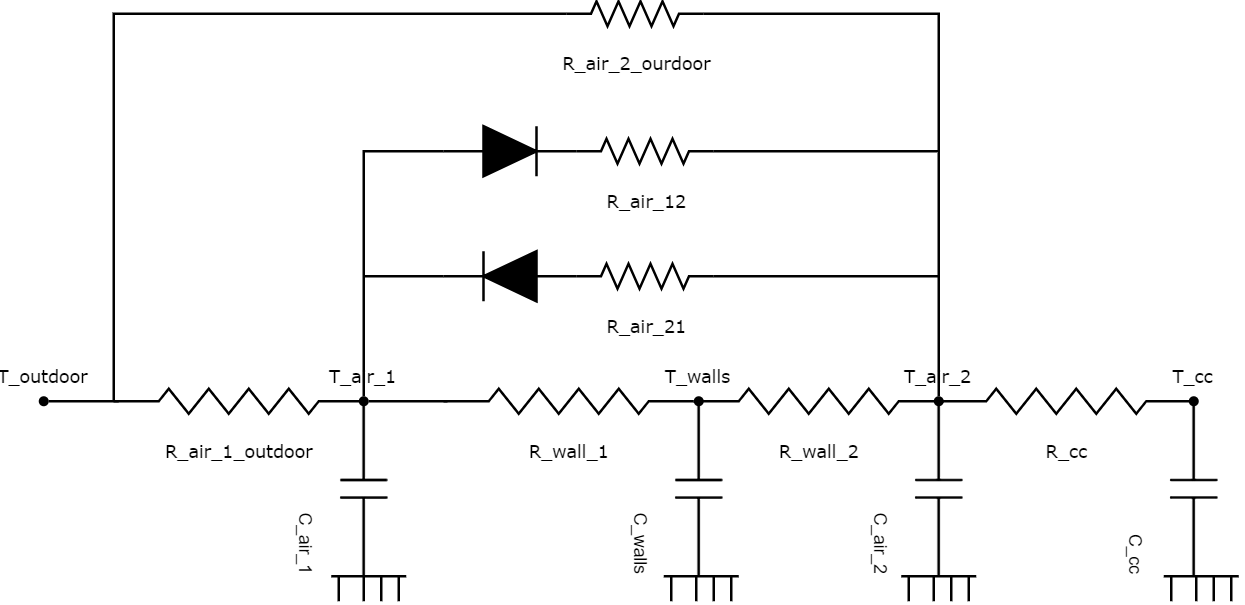
\includegraphics[width=1.0\columnwidth]{Pictures/2_Zones_house_circuits.png}
	\caption[Short title]{R-C circuits of 2 zones house model}
	\label{fig:elec7R4C}
	\end{figure}

with:\\
\begin{itemize}
    \item \texttt{T\_outdoor} : outdoor temperature [$\degr C$] 
    \item \texttt{T\_air\_1}  : zone 1 air temperature [$\degr C$]
    \item \texttt{T\_walls}   : wall temperature [$\degr C$]
    \item \texttt{T\_air\_2}  : zone 2 air temperature [$\degr C$]
    \item \texttt{T\_cc}      : temperature of the concrete layer between zone 1 and zone 2 [$\degr C$]
    \item \texttt{R\_air\_1\_outdoor} : outdoor resistance valus.
    \item \texttt{R\_wall\_1} : walls resistance value.
    \item \texttt{R\_wall\_2} : walls resistance value.
    \item \texttt{R\_cc}      : concrete resistance value.
    \item \texttt{R\_air\_12} : resistance value of air flow from zone 1 to zone 2.
    \item \texttt{R\_air\_21} : resistance value of air flow from zone 2 to zone 1.

\end{itemize}
\newpage

% \section{NEN and ISO}

The list of NEN and ISO standard used in the calculation:

\begin{itemize}
    \item NTA 8800
    \item NEN 1068
    \item ISO 6946
    \item ISO 10077-2
    \item NEN 7120
\end{itemize}

\newpage

\appendixname{A}\label{app:simulink}
\appendix
\section{Dwelling parameters calculation}
The initial parameters value for House model (row house 1975 to 1991) are listed in the table below\cite{VOORBEELD}:


\begin{table}[H]
    \centering
    
\begin{tabular}{|p{3cm}||p{7cm}||p{3cm}||p{3cm}|}
 \hline
 \multicolumn{4}{|c|}{Initial Parameters Value} \\
 \hline
\textbf{Abbreviation} & \textbf{Description} & \textbf{Value} & \textbf{Units}\\
 \hline
 
$A_{facade}$ & Envelope surface (facade + roof + ground)   & 160.2 &  $m^2$\\
 \hline

$A_{internal{\_}mass}$ & Floor and internal walls surface    & 170 & $m^2$\\
 \hline

 $V_{dwelling}$ & Internal volume & 275.6 &$m^3$\\
  \hline

 $R_{c, facade}$ & Thermal resistance for unit area (thermal insulation), R-value & 1.3 &  $\frac{m^2K}{w}$\\
  \hline

 $U_{glass}$& Window thermal transmittance, U-value & 2.9 &$\frac{W}{m^2K}$\\
 \hline

n & Ventilation, air changes per hour  & 0.55 & $[number/h]$\\

\hline

 CF& Convection factor & 0.8 &\\
 \hline
 
 $N_{facade}$ &Facade construction index & Light weight = 0/ Middle weight = 1/ Heavy weight = 2 &  \\
 \hline
 
  $th_{facade}$& Construction thickness: Light weight / Middle weight / Heavy weight  & [ 0.1,  0.1, 0.2 ] & m \\
 \hline
  
 $c_{facade}$& Specific heat capacity construction [J/kgK] & [840, 840, 840] &$\frac{J}{kg \cdot K}$\\
 \hline
 
 $\rho_{facade}$& Density construction: Light weight / Middle weight / Heavy weight  & [500, 1000, 2500] &$\frac{kg}{m^3}$\\
 \hline
 

 $N_{internal{\_}mass}$& Floor and internal walls construction index  & Light weight = 0/ Middle weight = 1/ Heavy weight = 2 &\\
 \hline
 
 $th_{internal{\_}mass}$& Construction thickness: Light weight / Middle weight / Heavy weight & [ 0.1,  0.1, 0.2 ] & m \\
 \hline
 
 $c_{internal{\_}mass}$& Specific heat capacity construction & [840, 840, 840] &$\frac{J}{kg \cdot K}$\\
 \hline
 
 $\rho_{internal{\_}mass}$& Density construction: Light weight / Middle weight / Heavy weight  & [500, 1000, 2500] &$\frac{kg}{m^3}$\\
 \hline
 
 $\rho_{air}$& Density air & 1.20 &$\frac{kg}{m^3}$\\
 \hline
  
 $c_{air}$& specific heat capacity air  & 1005 &$\frac{J}{kg \cdot K}$\\
 \hline
 
 $\alpha_{i{\_}facade}$ & Heat transfer coefficient. Surface Interior thermal resistance $R_{si} =\frac{1}{\alpha_{i{\_}facade}}$  (R\textsubscript{c}-waarde = 0.13, ISO 6946) & 8 & $\frac{W}{m^2 \cdot K}$ \\
\hline
 
 $\alpha_{e{\_}facade}$ & Heat transfer coefficient. Surface Exterior thermal resistance $R_{se} =\frac{1}{\alpha_{e{\_}facade}}$ (0,04 $\frac{m^2k}{W}$, ISO 6946, external surfaces or external side of exterior wall) & 23 &$\frac{W}{m^2 \cdot K}$\\
\hline
 
$\alpha_{internal{\_}mass}$& Heat transfer coefficient. Internal wall thermal resistance $ R_{air{\_}wall} =\frac{1}{A_{internal{\_}mass} \cdot \alpha_{internal{\_}mass}} $ Resistance indoor air-wall  & 8 &$\frac{W}{m^2 \cdot K}$\\
\hline
 
 $\rho_{internal{\_}masss}$& Density construction & [500, 1000, 2500] & $\frac{Kg}{m^3}$\\
\hline

\end{tabular}

\caption{Values of constants and parameters in house model.}
\label{tab:Paramteres}
\end{table}

\newpage
Volume floor and internal walls construction [$m^3$]: $V_{internal,mass} = A_{internal,mass} \cdot th_{internal,mass}$

Ventilation, volume air flow $[\frac{m^3}{s}]$: $qV = \frac{n \cdot V_{dwelling}}{3600} $  

Ventilation, mass air flow $[\frac{kg}{s}]$ : $qm = qV \cdot \rho_{air} $  
\newline

\textbf{Calculation of the resistances.}
\newline

Resistance indoor air-wall: $R_{air_{\_}wall} = \frac{1}{A_{internal,mass} \cdot \alpha_{internal,mass}} $ 

U-value indoor air-facade: $U =\frac{1}{\frac{1}{\alpha_{i{\_}facade}}   + R{c{\_}facade} + \frac{1}{\alpha_{e{\_}facade}}}$ 

Resistance indoor air-outdoor air: $R_{air{\_}outdoor} = \frac{1}{A_{facade} \cdot U + A_{glass} \cdot U_{glass} + qm \cdot c_{air}}$ 
\newline

\textbf{Calculation of the capacities.}
\newline
The heat capacity of interior walls can be determined using half of the actual wall thickness because both surfaces are considered as storing energy \cite{Architecture}.

Thermal capacity indoor air and walls: $C_{air} =\frac{rho_{internal{\_}mass} \cdot c_{internal{\_}mass} \cdot V_{internal{\_}mass}}{2} + \rho_{air} \cdot c_{air} \cdot V_{dwelling}  $ 

Thermal capacity walls : $C_{wall} =\frac{rho_{internal{\_}mass} \cdot c_{internal{\_}mass} \cdot V_{internal{\_}mass}}{2}$   

\newpage
  

%\appendixname{B}
\section{R and C Values explanation.}

In \cite{HTTHERMO} and \cite{FUND} the expressions in Fig.\ref{table_1} are derived.
For conduction, the expression for $R_{th} = \frac{L}{k\dot A}$


The units of $R_{th}$ are: $ [\frac{K}{W}] $

$ [W] = [\frac{W}{m \cdot K}] \dot [m^2] \cdot [\frac{K}{m}] $

The units of $k$ are: $ [\frac{m}{m^2} \cdot \frac{W}{K}] = [\frac{W}{m \cdot K}]$

Thermal conductivity of material $k = [\frac{W}{m \cdot K }] = [\frac{W}{m \cdot K }]  = [W \cdot m^{-1} \cdot K^{-1}]$

$k$ is also denoted as $\lambda$

Reference: \cite{ELECRESCOND}

Ohm's Law: $ R = \frac{U}{I} \quad [\frac{V}{A}] = [\Omega] $

Electrical resistivity: $ \rho = [\frac{\Omega \cdot m^2}{m} ] = [\Omega \cdot m] $ Material property.

Electrical conductivity: $ \sigma = \frac{1}{\rho} =[\frac{1}{\Omega \cdot m}] = [\frac{S}{m}] $ Material property.

Electrical resistance $ R = \frac{\rho \cdot L}{A} $ or $ R = \frac{L}{\sigma \cdot A} $
\\

Thermal Law: 
Heat flux $ \dot Q $ in $ [W \cdot m^{-2}] $

$ \dot Q = \frac{\Delta T}{R_{th}} \quad R_{th} = \frac{\Delta T}{\dot  Q} 
\quad [\frac{K}{W \cdot m^{-2}}] = [\frac{m^2 \cdot K}{W}]$

(Specific) Thermal resistivity: $ R_\lambda $ or $ r = [\frac{K}{W \cdot m^{-2}} \frac{1}{m} ] = [\frac{m \cdot K}{W}] $ Material property.

Thermal conductivity: $ \lambda $ or $ k  = \frac{1}{r} = [\frac{ W \cdot m^{-2} }{K} \cdot m] 
= [\frac{W}{m \cdot K}] $ Material property

Thermal resistance R-value or $ R_{th} = \frac{r \cdot L}{A} $ or $ R = \frac{L}{k \cdot A} $

Unit $ R_{th} = [\frac{m \cdot K}{W} \frac{m}{m^2}] = [\frac{m^2 \cdot K}{W}] $
\\

$R_c$-value $ = r \cdot L = \frac{L}{k} = \frac{L}{\lambda} $

\newpage


\appendixname{C}
\section{NEN and ISO}

The list of NEN and ISO standard used in the calculation:

\begin{itemize}
    \item NTA 8800
    \item NEN 1068
    \item ISO 6946
    \item ISO 10077-2
    \item NEN 7120
    \item NEN 5060\cite{NEN5060}
\end{itemize}

\newpage

%\bibliography{mybibliography}
\printbibliography[heading=bibintoc]

\end{document}



